\subsection{Communication Layer}
\label{sec:communication-layer}
% introduction to communication layer
The sub-systems of VRDAVis need communication channels and protocols to communicate effectively.
These channels are established between the components of the front-end service and remote services. 
The data and signalling servers within the remote services communicate with the client application in the front-end. 
Peer-to-peer connections are formed between instances of the client within front-end services. 

\subsubsection{Data Server and Desktop/VR Client Application}
The communication between the user-side browser application and the server-side data server takes place through a WebSocket connection, which is more suitable for VRDAVis than the typical request and response or promise and resolve model common in many HTTP-based clients and servers~\cite{MDN_WebSockets_API}.
WebSockets allow the respective systems to send messages to each other without requiring a request first to respond. 
This behaviour allows for many responses to a single request, 
so the server is not restricted to responding to the client with a single very large message with a large piece of data, it can send smaller pieces of data in individual messages.

Protocol Buffers are used to define the structure of messages and facilitates the reading and writing of structured data to and from various data streams using different programming languages, such as C++, JavaScript, and Python.
The Protocol Buffer library was created by Google to serialise structured data. 
A platform-neutral mechanism for converting data objects into a byte stream for transfer~\cite{Google_Protocol_Buffers}.
This library is used to define a schema and format for data exchanged between the front-end and remote services. 
The Protocol Buffer message definitions are stored in their own folder and are used by the user-side and server-side systems. 
When a message needs to be sent from the user-side to the server-side or vice versa, the data objects are serialised into a byte stream before they are transferred. 
Once the data arrives, it is converted from a byte stream back into a data object.
% serialisation -> process of converting data type objects into a byte stream for transfer
IProtocol Buffers was chosen for its error-prevention capabilities compared to JavaScript Object Notation (JSON), and because it is the chosen communication format used in CARTA.

\subsubsection{Signalling Server and Desktop/VR Client Application}
The signalling server creates, manages, and establishes peer-to-peer connections between instances of the client browser application on different devices.
% JSON
The communication required between the signalling server and the client application is significantly less complex than the communication between the data server and the client application.
The tasks performed by the signalling server are also less time-sensitive than those performed by the data server, and less data needs to be transferred between them.
These factors led to the use of the simple request-response communication protocol to be used as well as the use of JSON to format the messages.
JSON is a lightweight format for storing and transporting data that is language-independent and easy to understand as it considered ``self-describing"~\cite{JSON}.

\subsubsection{Client Application and Client Application}
Another component of the communication layer is the peer-to-peer connection between two instances of the client web browser application. 
One of these instances would be in a browser on a desktop computer, and the other would be in the browser on a standalone VR headset. 

Web Real-Time Communication (WebRTC)~\cite{Blum2021, WebRTC} is an internet communication protocol that enables web applications to stream audio, video, or data between peer browser windows, without the need for the data to be routed through an intermediate server. 
It facilitates peer-to-peer communication without requiring additional third-party packages.
% facilitates peer-to-peer without requiring plug-ins or third-party software to be installed
% support for audio and video conferencing, file exchange, screen sharing, identity management, and interfacing with legacy telephone
WebRTC is used in VRDAVis to establish a connection between these instances. 
This connection is used to transmit the application's state between its peers, allowing the user to continue their work seamlessly without needing to repeat steps on another device.
% used to create a peer-to-peer connection between browser instances on different devices
% used to send data between the broswer instances 
% chosen for its functinality to create peer-to-peer connections
% peer-to-peer connection
This peer-to-peer connection allows the instances to exchange data between instances without having to send it through middleware service such as a server. 
However, it does require the signalling server to establish and manage the connections. 

% has the capability with help from the signalling server to create a peer-to-peer conection between another instance of the client on a VR headset
%   show pairing process diagrams
%   show transfer diagram

\paragraph{Headset Pairing}
% To establish the connection both devices must connect to the signalling server which a server-side component which stores unique id pairs which.
The initial pairing process requires both of the VR headset and the desktop computer to be connected to the signalling server. 
When each devices connects, it sends the server an unique ID, a name, and announces whether it is a VR capable device. 
The server checks if the device already has a pair and if it does not find a pair it sends a list of unpaired VR devices to the unpaired devices which are not VR-capable. 
A desktop user selects a VR device and generates a code from the desktop computer, a code which is sent to the signalling server, and forwarded to selected device using its unique ID. 
The VR device then prompts the user to enter the code locally, and verifies it against the code received from the server.
When the server confirms that the codes match it saves the device pair to a local JSON database.
The server then sends a confirmation message to both devices stating that the devices have been paired.
Both devices then confirm that they are ready to begin a peer-to-peer connection and the WebRTC peer-to-peer protocol begins.

\begin{figure}
    \centering
    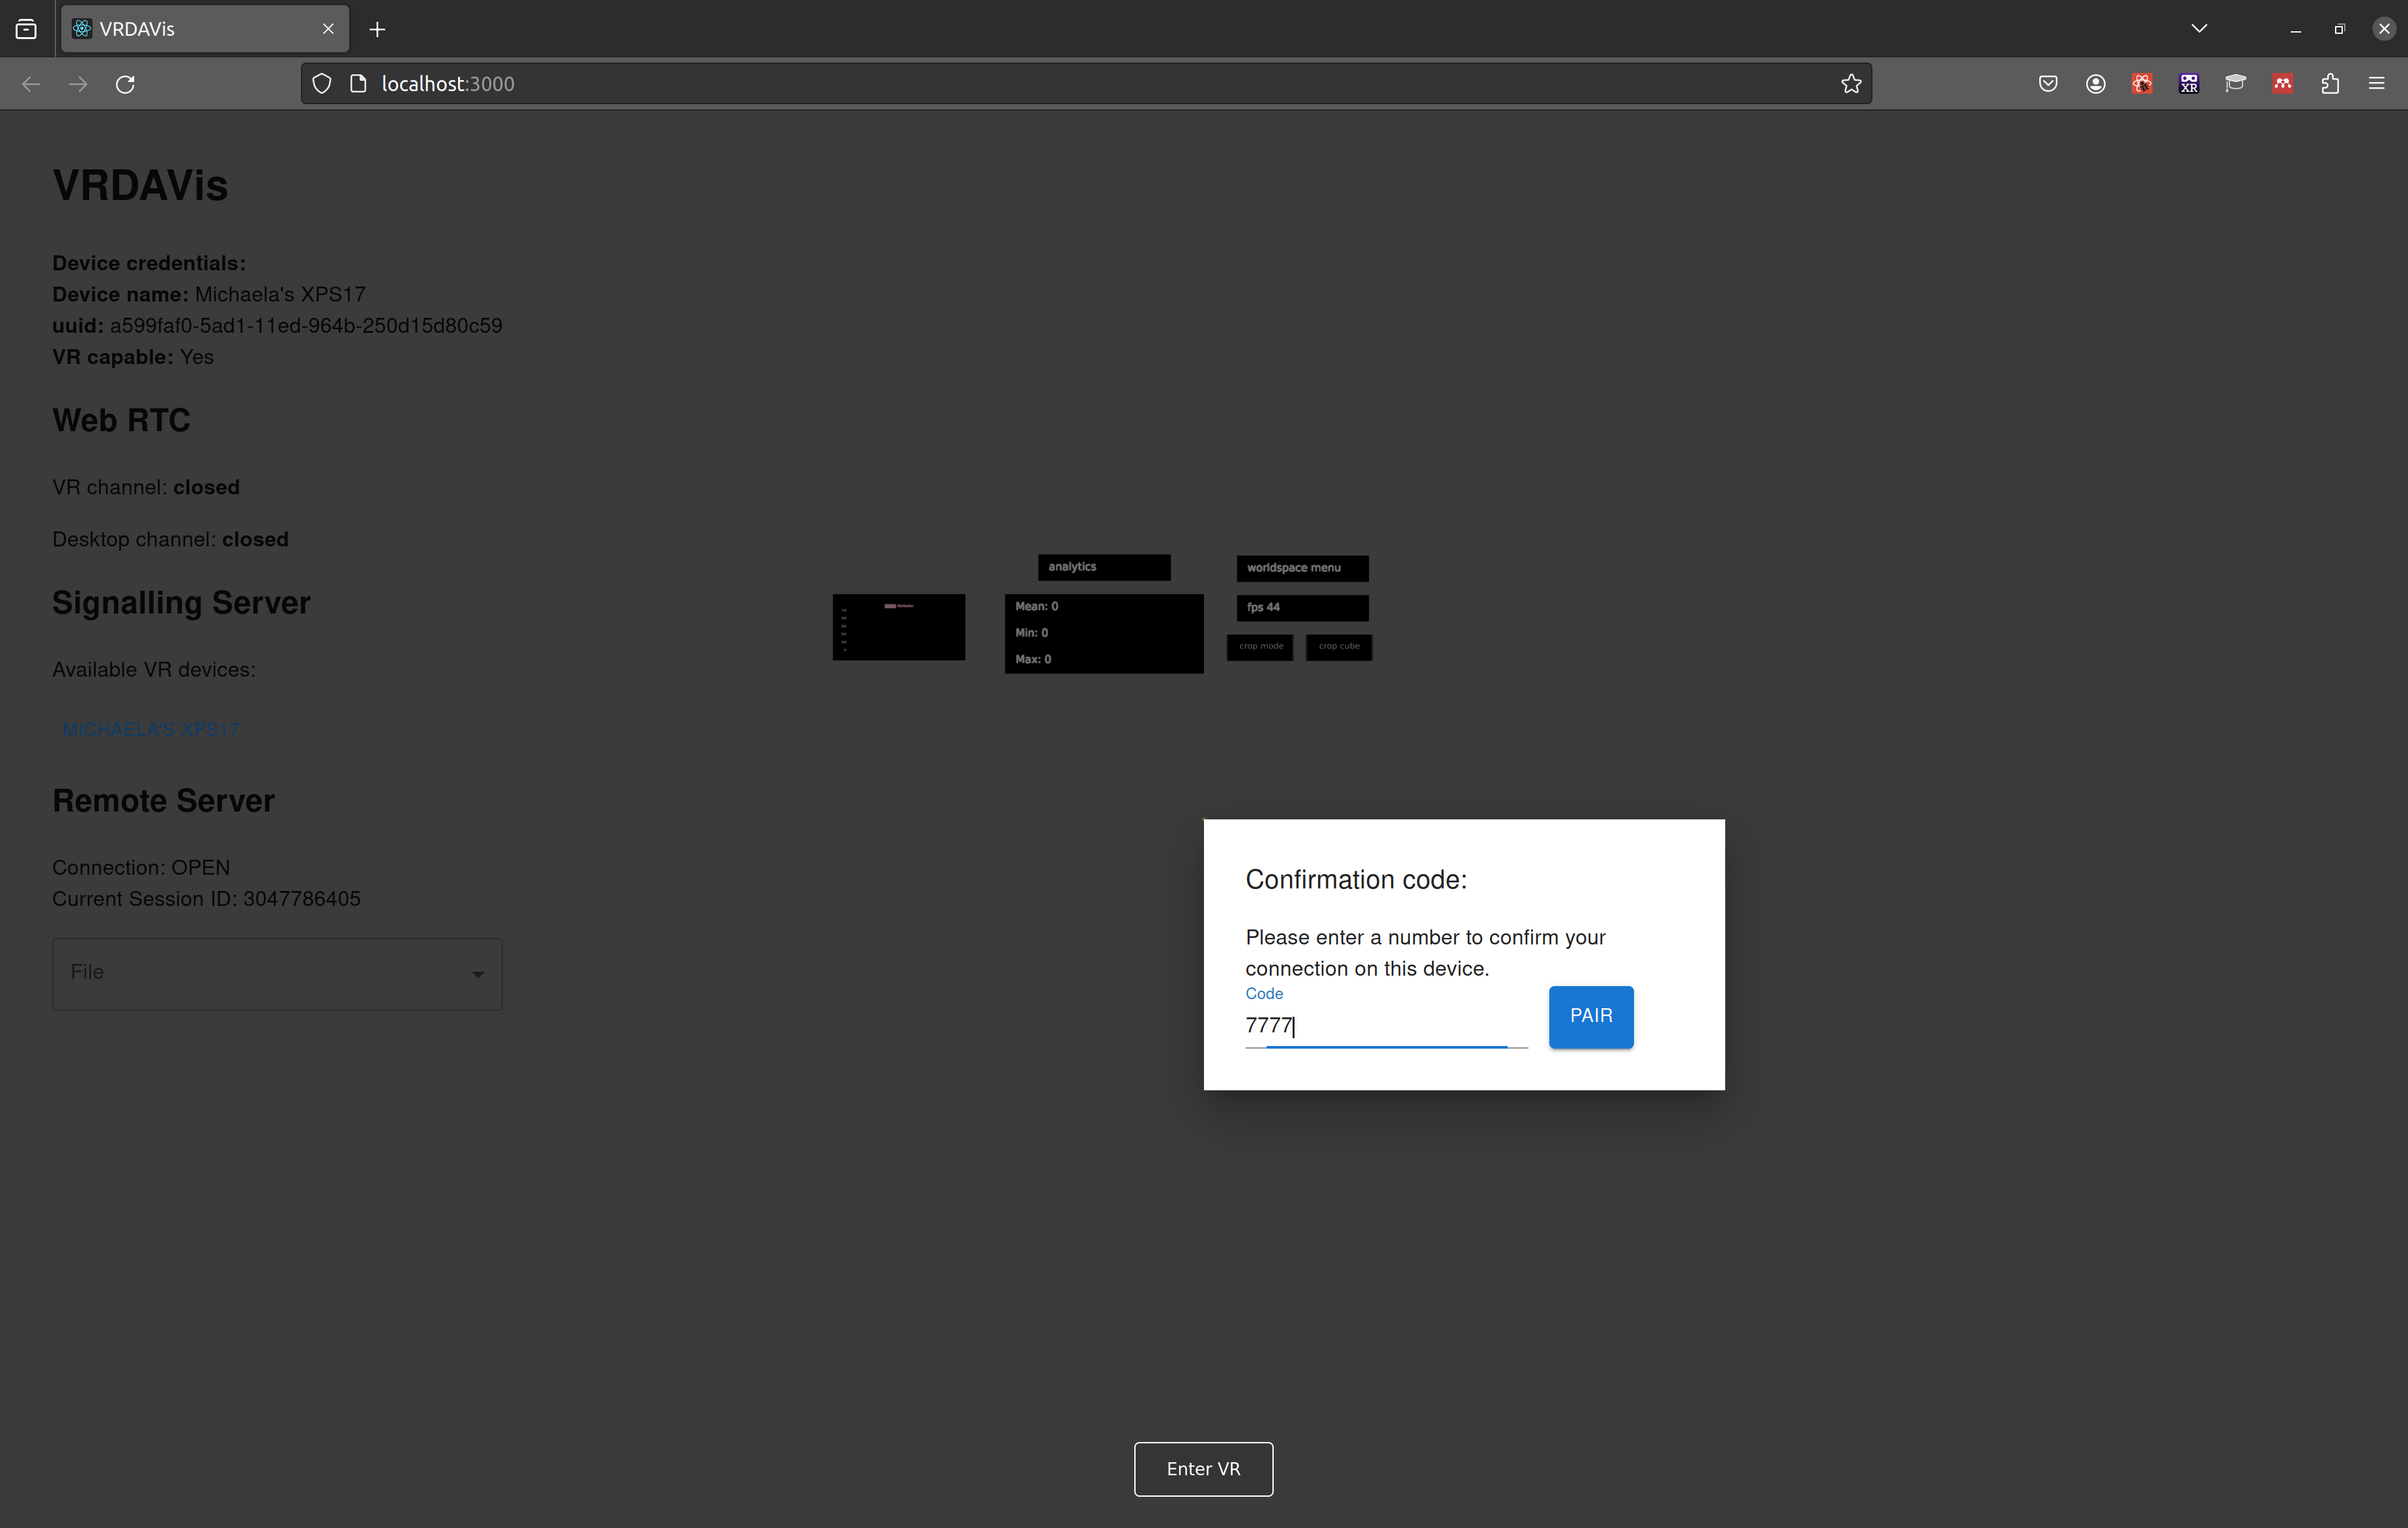
\includegraphics[width=\linewidth]{figures/screenshots/3.png}
    \caption{The menu that appears in the browser window when the user selects a VR device to pair with on the desktop computer. The user must enter a code which must also be entered in the same menu on the VR headset.}
    \label{fig:screenshot-3}
\end{figure}

% pairing process diagrams
\begin{figure*}
    \centering
    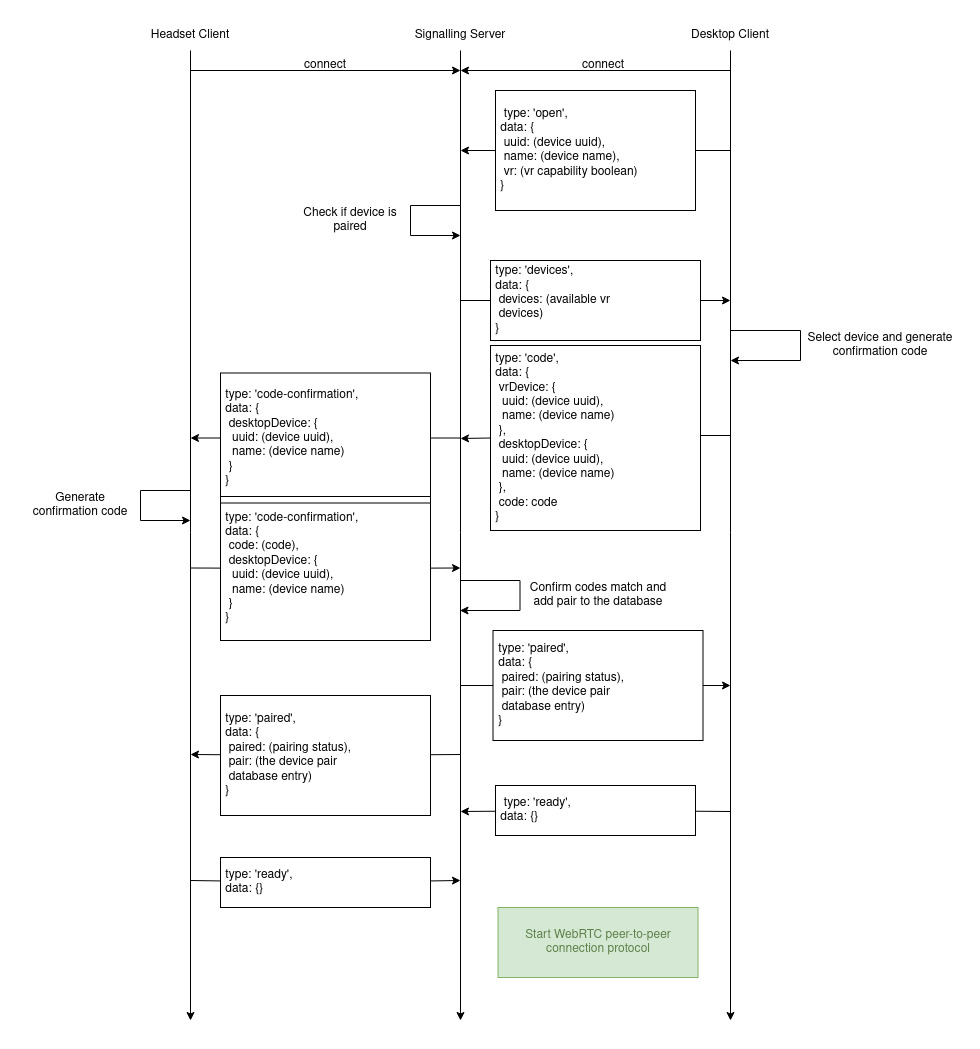
\includegraphics[width=0.6\linewidth]{figures/pairing-process.jpg}
    \caption{The pairing process between an instance of the front-end application running on a desktop computer and an instance running on a VR headset. It shows the order of the messages sent from each device and the contents of each message.}
    \label{fig:pairing-process}
\end{figure*}

\paragraph{Paired Devices Connection}
% Once the devices have been paired they must connect to the signalling server at the same time and then a peer-to-peer connection is established between the paired devices. 
% No data which is sent between the devices on the peer-to-peer connection passes through this server.
When one device connects to the signalling server, the server checks if the device is currently paired by searching the JSON file which contains all the pairs.
If the device is paired, the server checks if the other paired device is connected to the server as well.
When the VR device and the desktop computer are connected to the signalling server and the server detects that these device are paired to each other, it starts the process of creating the WebRTC peer-to-peer connection.

\begin{figure*}
    \centering
    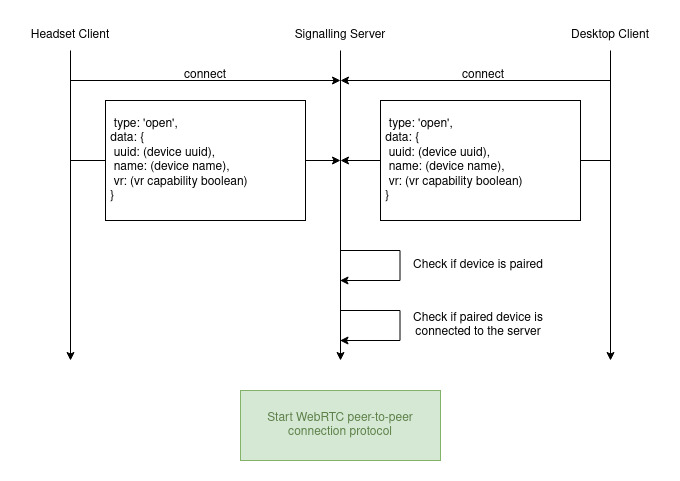
\includegraphics[width=0.6\linewidth]{figures/connect-paired-devices.jpg}
    \caption{The process of connecting paired devices through the signalling server. Both devices indicate that they wish to open a peer-to-peer connection with their ``open" messages.}
    \label{fig:connect-paired-devices}
\end{figure*}

\paragraph{Peer-to-peer Connection}

Once the VR headset and the desktop client indicate that they are ready to establish a peer-to-peer connection with each other,
the desktop client sends WebRTC Interactive Connectivity Establishment (ICE) candidates to the VR device through the signalling server.
These ICE candidates contain the protocols and routing needed for remote devices to communicate with each other as well as details used to establish the connection.
Multiple candidates are sent until one is found which works for both devices.
The candidates are sent to the VR device through the signalling server as this is the only channel currently connecting the devices.
The desktop computer creates a Session Description Protocol (SDP) offer, which contains the RTCPeerConnection interface. 
It contains information about open channels already attached to the current WebRTC session, a codec, any candidates already gathered, and options supported by the browser.
This SDP offer is sent to the VR device through the signalling server, and the VR device handles the offer through WebRTC by creating an answer which contains the corresponding information about its own capabilities.
The answer is returned to the desktop client, the offer is resolved and the peer-to-peer connection is established between the devices.
No further data needs to pass through the signalling server in order for the devices to communicate with each other; they now pass data to one another through the peer-to-peer connection.

\begin{figure*}
    \centering
    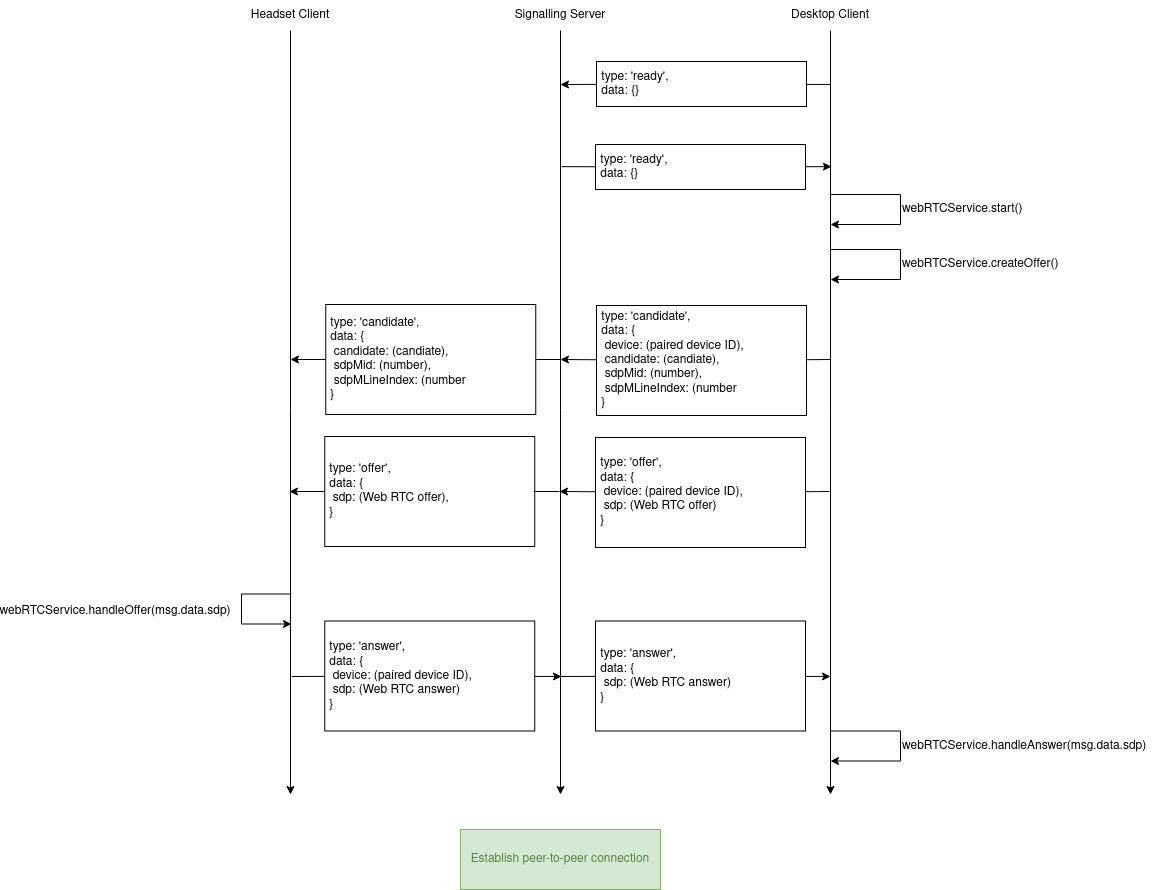
\includegraphics[width=0.8\linewidth]{figures/peer-connection(1).jpg}
    \caption{How the peer-to-peer connection is established between the paired devices.}
    \label{fig:peer-connection}
\end{figure*}

\paragraph{Transferring Client Application State Over Peer Connection}
The purpose of the peer-to-peer connection is for the connected instances of the front-end to exchange state.
This allows the user to start their exploration of a data cube on a device such as a laptop or a desktop computer, then move the state of the desktop instance to the VR headset to continue the exploration in the VR environment.
Transferring the state of an instance in this manner means that the user does not need to perform additional steps to start a new instance and get back to the same position in their new exploration.

The state is transferred through JSON messages sent over the peer-to-peer connection.
Each message contains the file name, and the size and the position of the local cube state.
Once these details have reached the new instance, a new connection to the data server is used to make requests and receive responses from.

% JSON
% add a diagram for how the state is transferred between the devices
\begin{figure*}
    \centering
    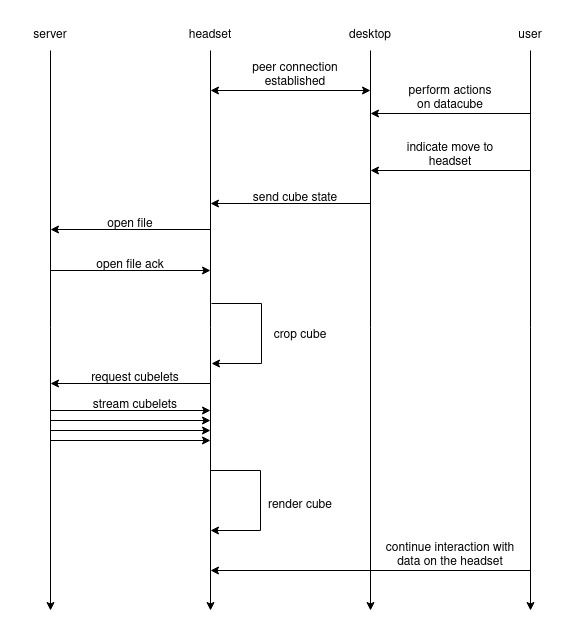
\includegraphics[width=0.6\linewidth]{figures/transfer-flow.jpg}
    \caption{The diagram depicts the event sequence for transferring the state between the two instances of the front-end browser application. The application state can be bilaterally transferred between client devices.}
    \label{fig:transfer-flow}
\end{figure*}

\begin{figure*}
    \centering
    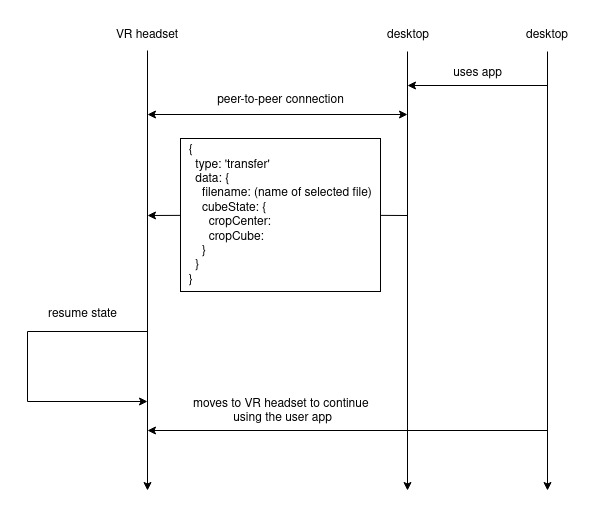
\includegraphics[width=0.6\linewidth]{figures/transfer-cube-state.jpg}
    \caption{The message structure which is sent between the VR headset instance and the desktop instance when the cube state needs to be transferred between the devices.}
    \label{fig:transfer-cube-state}
\end{figure*}
